\documentclass[conference]{IEEEtran}
\IEEEoverridecommandlockouts
% The preceding line is only needed to identify funding in the first footnote. If that is unneeded, please comment it out.
\usepackage{cite}
\usepackage{amsmath,amssymb,amsfonts}
\usepackage{algorithmic}
\usepackage{graphicx}
\usepackage{textcomp}
\usepackage{xcolor}
\usepackage{hyperref}
\def\BibTeX{{\rm B\kern-.05em{\sc i\kern-.025em b}\kern-.08em
    T\kern-.1667em\lower.7ex\hbox{E}\kern-.125emX}}
\begin{document}

\title{Mamba-Based Tumor Segmentation\\
\thanks{$\dagger$ Equal contributions}
}

\author{\IEEEauthorblockN{Clay Crews$^{\dagger}$}
\IEEEauthorblockA{\textit{Department of Computer Science} \\
\textit{University of South Carolina}\\
Columbia, SC, United States \\
jccrews@email.sc.edu}
\and
\IEEEauthorblockN{Lexington Whalen$^{\dagger}$}
\IEEEauthorblockA{\textit{Department of Computer Science} \\
\textit{University of South Carolina}\\
Columbia, SC, United States\\
LAWHALEN@email.sc.edu}
}

\maketitle

\begin{abstract}
U-net and transformer-based architectures have dominated medical image segmentation, particularly for tumor segmentation from brain MRI scans. However, Structured State Space Sequence Models (SSMs), as highlighted by Gu, Goel, and Ré, present a promising alternative with comparable modeling power to transformers but linear scalability in sequence length, making them well-suited for large medical images.

We propose exploring the application of the Mamba block, a variant of SSMs, for tumor segmentation in brain MRI scans. By leveraging selective state spaces, Mamba blocks can potentially enhance the efficiency and effectiveness of tumor segmentation while maintaining linear scalability.

Our methodology involves implementing and fine-tuning a Mamba-based architecture on a dataset of annotated brain MRI scans. We will evaluate the model's performance using standard segmentation metrics and compare the results with U-net and transformer-based approaches.
\end{abstract}

\begin{IEEEkeywords}
Mamba, Segmentation, Selective State Spaces
\end{IEEEkeywords}

\section{Introduction}
MRI imaging to identify brain tumors has naturally been a target for accurate image segmentation through the use of ML architecture. The use of computer-aided diagnosis of tumors can be crucial to quickly identify tumors and determine a course of action for the patient. Gliomas are the most common primary brain malignancy with varying degrees of aggressiveness in the brain. The protocol for MRI image annotation of these tumors consists of the following labels: the whole tumor extent, the tumor core, the non-enhancing/necrotic tumor region, and regions of low grade gliomas \cite{bakas2019identifying}. These annotations of an MRI are used to determine the size and severity of a tumor.
	
To accurately segment these images, picking out the small features of the image becomes the focus. The use of the U-Net architecture, presented by Ronneberger, Fischer, and Brox \cite{ronneberger2015unet}, has had success in MRI image segmentation. U-Net builds on the approach of fully convolutional networks by improving the limitation on the large amount of data needed to accurately train the model. Very few training images are needed due to the contracting and expansive paths in this architecture. In the contracting path, images are downsampled and pooled along with increasing the number of feature channels. Each downsampled resolution produces a multi-channel feature map. The expansive path up samples and combines with each segmentation feature map from the contracting layer to localize features in the image. A 1x1 convolution layer is applied to the final image to map the large feature vector to a selected number of classes. All of this essentially creates a feature map where each pixel’s relevance is taken into account and evaluated in the end result. An approach using the U-Net architecture would provide the detailed analysis needed for tumor annotation. 

An arising issue in the complex recurrent or convolutional neural networks used for image segmentation is the length of the sequences given as input. Maintaining relevance of the current area of an image in relation to the rest of the image is key for more accurate segmentation. An approach with the Transformer architecture has a large emphasis on learning specific features in an image, outlined by Vaswani et al. 2017 \cite{vaswani2023attention}. This architecture follows an encoder-decoder pattern, connected through an attention mechanism, a transformer block. Transformer blocks show capability of learning long-distance dependency throughout an input image. In the self-attention mechanism for this block, a single element in a given sequence is compared to all of the elements in the sequence. However, this mechanism becomes computationally very expensive when it comes to long sequences.
	
Selective State Spaces (SSMs) pose an improvement in computational efficiency over Transformers for this long dependency range. SSMs represent the relevance and context of different parts of the input sequence giving selective attention. This model is widely used in control theory for time variant systems and in fields such as computational neuroscience. Selective attention is very efficient in handling long sequences over time and presents a more localized context of the data. Sections of sequences that deserve attention are represented by the model and will dynamically update these values to reflect the contextual relevance. 
	
Making use of Structured State Spaces, presented by Gu, Goel, and Ré \cite{gu2022efficiently}, for their superiority in long range dependency tasks, a specific type of SSM, the Mamba architecture, by Gu and Dao \cite{gu2023mamba}, proposed a foundational model to operate on arbitrary sequences from a variety of inputs in the domain of sequence modeling. This model achieves the power of Transformers while scaling linearly in sequencing length to be computationally efficient. Additionally, the selection mechanism of Mamba improves on an SSMs ability to focus on or ignore sections in an input sequence by parameterizing the parameters of an SSM to reflect the current context of the input. The Mamba model and its application to brain tumor MRI imaging segmentation will be evaluated in this project.

\section{Input Data}\label{sec2}
We shall be using a Brain MRI segmentation dataset found here in \cite{dataset}. This dataset has been used in several papers regarding classification of the shape and severity of tumors, and provides an adequate dataset for research purposes in the field of medical image analysis, particularly in the area of brain MRI segmentation. Researchers have utilized this dataset in various studies focusing on the classification of tumor shapes and the assessment of tumor severity. With its comprehensive collection of brain MRI scans, along with corresponding segmentation masks, the dataset offers valuable resources for developing and evaluating algorithms aimed at automating tumor detection and analysis.

The dataset contains brain MRI images along with their segmentation masks for 110 patients, for a total of almost 4000 total images, of which about 1400 have tumors.


\section{Output Data}\label{sec3}
The output of this model shall be segmentation masks for new, never before seen images. 

\section{Compared Models}
Prior to an analysis of how the Pyramidal U-Mamba compares, we shall explain what models we chose for comparison and why.

For this our analysis, we compare four models against our's. The models are U-Net\cite{ronneberger2015unet},ResNet18, ResNet50, U-Mamba\cite{U-Mamba}, and SegViT\cite{dosovitskiy2021image}. Below we explain our choices.
\subsection{U-Net}
 The core idea behind U-Net is to complement a traditional contracting network with successive layers that replace pooling operations with upsampling operators. These upsampling layers aim to increase the resolution of the output. Subsequent convolutional layers can then learn to assemble a precise output based on this high-resolution information [1]. 
 A key modification in the U-Net architecture is the inclusion of a large number of feature channels in the upsampling part. This allows the network to effectively propagate contextual information to higher resolution layers. As a result, the expansive path of the network becomes more or less symmetric to the contracting part, leading to a distinctive U-shaped architecture. Unlike traditional convolutional networks, U-Net does not employ any fully connected layers and only utilizes the valid part of each convolution [2]. To predict pixels at the border regions of the image, the missing context is extrapolated by mirroring the input image. This tiling strategy is crucial for applying the network to large images, as it circumvents resolution limitations imposed by GPU memory constraints \cite{ronneberger2015unet}. Due to its encoder-decoder architecture, skip connections, multi-scale feature extraction, and its efficiency, U-Net has been used in many denoising and diffusion models. For instance, DDPMs (Denoising Diffusion Probabilistic Models) use an architecture similar to U-Net for denoising and sample generation \cite{DBLP:journals/corr/abs-2006-11239} while the popular Stable Diffusion architecture uses a U-Net based architecture for the diffusion process \cite{rombach2021highresolution}. We have chosen to compare our novel segmentation architecture against the U-Net architecture due to its well-established reputation and widespread adoption in the field of medical image segmentation.
 

\subsection{ResNet}
We have also selected ResNet18 and ResNet50 as additional benchmarks. These architectures, introduced by He et al. in their seminal work "Deep Residual Learning for Image Recognition" \cite{DBLP:journals/corr/HeZRS15}, have revolutionized the field of deep learning by addressing the problem of vanishing gradients in deep neural networks. The key innovation in ResNets is the introduction of residual connections, which allow the network to learn residual functions with reference to the input layer, thereby facilitating the training of much deeper networks. ResNet18 and ResNet50, with 18 and 50 layers respectively, have been widely adopted in various computer vision tasks, including image classification, object detection, and segmentation. These models have demonstrated exceptional performance and generalization ability across diverse datasets. By comparing our proposed architecture against ResNet18 and ResNet50, we aim to assess its effectiveness in relation to these well-established and highly influential architectures. This comparison will provide valuable insights into the capabilities of our model and its potential to advance the state-of-the-art in image segmentation tasks.
\subsection{U-Mamba}
As our model takes much inspiration from the recently developed U-Mamba design \cite{U-Mamba}, we also choose to incorporate it in our comparison. U-Mamba addresses these limitations by introducing a novel hybrid CNN-SSM block that leverages the strengths of both architectures. The convolutional layers in the block are responsible for local feature extraction, while the State Space Sequence Models (SSMs) (Gu et al., 2022), a new family of deep sequence models, are known for their strong capability in handling long sequences and capturing long-range dependencies. By integrating these two components, U-Mamba achieves a balance between local and global information processing, enabling it to effectively handle long-range dependencies in biomedical image segmentation tasks. Moreover, U-Mamba incorporates a self-configuring mechanism that allows it to automatically adapt to various datasets without manual intervention, enhancing its versatility and usability.
\subsection{SegViT}
SegViT \cite{zhang2022segvit} explores the capability of plain Vision Transformers (ViTs) \cite{dosovitskiy2021image} for semantic segmentation, leveraging the attention mechanism to generate masks for semantic segmentation. Unlike previous ViT-based segmentation networks that learn pixel-level representations from the output of the ViT, SegViT introduces the Attention-to-Mask (ATM) module. In the ATM module, the similarity maps between a set of learnable class tokens and the spatial feature maps are transferred to the segmentation masks, enabling effective semantic segmentation.
SegViT has demonstrated impressive performance on several benchmark datasets, including ADE20K, COCO-Stuff-10K, and PASCAL-Context, achieving state-of-the-art results. Moreover, to address the computational cost associated with the ViT backbone, SegViT proposes query-based down-sampling (QD) and query-based up-sampling (QU) to build a Shrunk structure. By comparing U-Mamba against SegViT, we aim to evaluate the effectiveness of our hybrid CNN-SSM approach in relation to the attention-based segmentation mechanism employed by SegViT. This comparison will provide insights into the strengths and weaknesses of both architectures and their ability to handle complex biomedical image segmentation tasks. Furthermore, it will help us understand the potential of attention mechanisms and hybrid approaches in advancing the state-of-the-art in biomedical image segmentation.

\subsection{UltraLight VM-UNet}
The UltraLight VM-UNet \cite{ultralightvmunet} is a lightweight neural network architecture designed for skin lesion segmentation tasks. It is built upon the Vision Mamba module, which is a state-space model (SSM) that can efficiently handle long-range dependencies in sequences, making it well-suited for image segmentation tasks.

The key innovation of the UltraLight VM-UNet is the proposed Parallel Vision Mamba Layer (PVM Layer), which processes deep features in parallel using multiple Vision Mamba blocks. Specifically, the input feature map is split into multiple sub-feature maps, each processed by a separate Vision Mamba block with a reduced channel count. This parallel processing approach allows the UltraLight VM-UNet to maintain high segmentation performance while significantly reducing the number of parameters and computational complexity.

The UltraLight VM-UNet is reported to have only 0.049 million parameters and a computational cost of 0.060 GFLOPs, which is significantly lower than traditional convolutional neural networks and transformers used for image segmentation tasks. Despite its lightweight nature, the authors demonstrate that the UltraLight VM-UNet achieves competitive performance on three publicly available skin lesion segmentation datasets, outperforming several state-of-the-art lightweight models.

The success of the UltraLight VM-UNet can be attributed to the authors' in-depth analysis of the key factors influencing the parameters of the Vision Mamba module. By identifying the number of input channels as a critical factor affecting the parameter count, they were able to design the PVM Layer to process features in parallel while keeping the overall channel count constant, leading to a significant reduction in parameters without compromising performance.

\section{Our Models}

Inspired by \cite{U-Mamba} and \cite{ultralightvmunet}, we sought to implement both models on a different problem: tumor segmentation.

Our goal was to 1) maintain dice scores comparable to state-of-the-art (SOTA) methods such as those listed above, while 2) being smaller than those above.

We now go into what we did for each of our models.


\subsection{PP-UMamba}
This model incorporates pyramidal pooling, which is a strategy used in convolutional neural networks (CNNs) to capture context and incorporate multi-scale information \cite{zhao2017pyramid}. Pyramidal pooling involves parallel pooling operations at different scales, followed by concatenation of the resulting feature maps. This approach has been shown to improve the performance of CNNs in various computer vision tasks, including segmentation, by enabling the model to capture both local and global context.

In our PP-UMamba model, we integrated pyramidal pooling into the U-Mamba architecture, aiming to leverage the strengths of both the Mamba module and multi-scale feature extraction.

\subsection{ULMUNet\_v1}
For ULMUNet\_v1, the initial channel list was modified from [8, 16, 24, 32, 48, 64] to [16, 32, 64, 128, 256], increasing the number of channels at each step of the encoder and decoder. Additionally, the depth of the U-Net was reduced by one layer to keep the parameter count low while increasing the number of parameters in each step. The intention was to improve performance by increasing the capacity of the model while maintaining a reasonable parameter count.

\subsection{ULMUNet\_v2}
In ULMUNet\_v2, the number of parallel branches in the Parallel Vision Mamba (PVM) block was increased from 4 to 8. This modification directly decreases the parameter count, further proving the idea proposed in the UltraLight VM-UNet paper \cite{ultralightvmunet} that processing features in parallel with reduced channel counts can significantly reduce parameters while maintaining performance.

\subsection{ULMUNet\_v3}
ULMUNet\_v3 combines the modifications from ULMUNet\_v1 and ULMUNet\_v2. It increases the number of parallel branches in the PVM block to 8 and modifies the channel list to [16, 32, 64, 128, 256]. Additionally, the depth of the U-Net was reduced to 5 layers. This approach aims to balance the trade-off between model capacity and parameter efficiency.

\subsection{ULMUNet\_v4}
This model incorporates pyramidal pooling, similar to PP-UMamba, but within the UltraLight VM-UNet architecture. The goal was to leverage the benefits of multi-scale feature extraction while maintaining the parameter efficiency of the UltraLight VM-UNet.

\subsection{UL-PP}
The UL-PP (Ultra Light Pyramidal Pooling) model trained and performed well with 1.1M parameters. Incorporating pyramidal pooling on the UL network scored slightly worse than without pyramidal pooling but required approximately 400,000 more parameters.

\begin{figure}[!t]
    \centering
    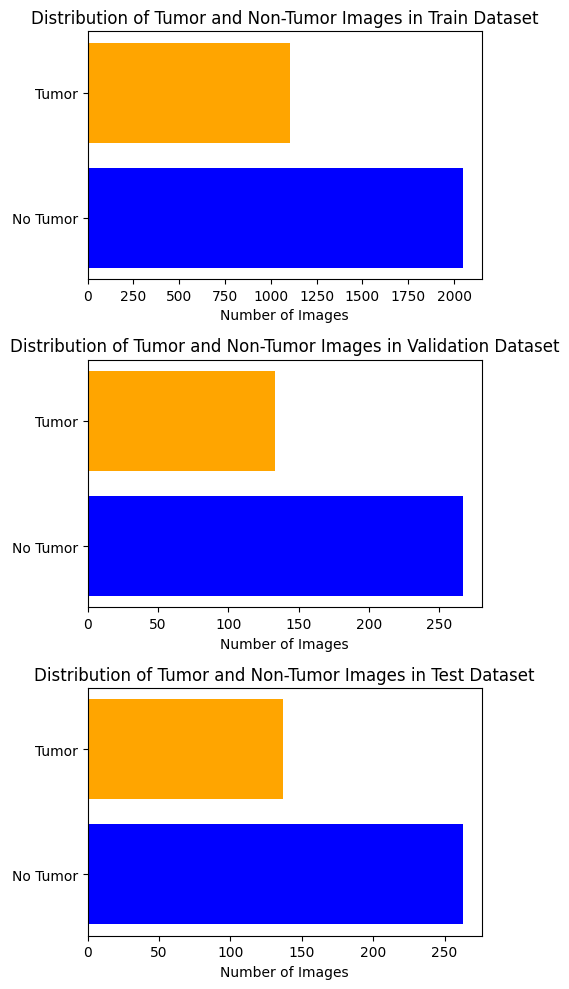
\includegraphics[width=\columnwidth]{imgs/data_stats.png}
    \caption{Information about the train, test, and validate data.}
    \label{fig:datastats}
\end{figure}

\section{Results}
We now compare our models against ResNet18, ResNet50, standard U-Mamba with bottleneck, UNet, and UltraLight VM-UNet. We train for 100 epochs on all models, and use dice-loss with Adam optimizer. We train on roughly 3000 images, and validate on roughly 400. we then test on roughly 400. We show the stats of our data in Figure \ref{fig:datastats}.
The results are shown in Figures \ref{fig:bars},\ref{fig:balls},\ref{fig:segs}.

\begin{figure}[!t]
    \centering
    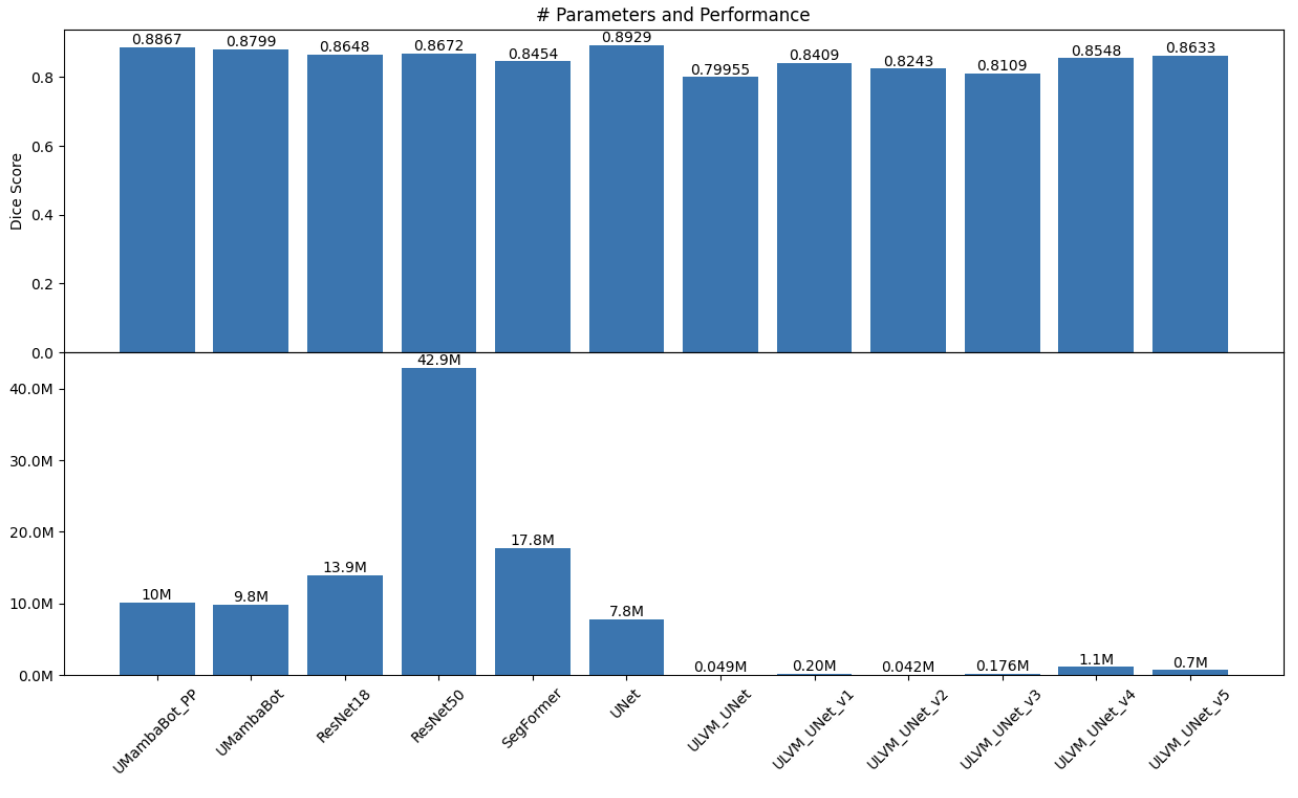
\includegraphics[width=\columnwidth]{imgs/bars.png}
    \caption{Each model tested as a bar chart. The upper half is the Dice Scores, and the bottom half is the parameter count, where M means "million".}
    \label{fig:bars}
\end{figure}
\begin{figure}[!t]
    \centering
    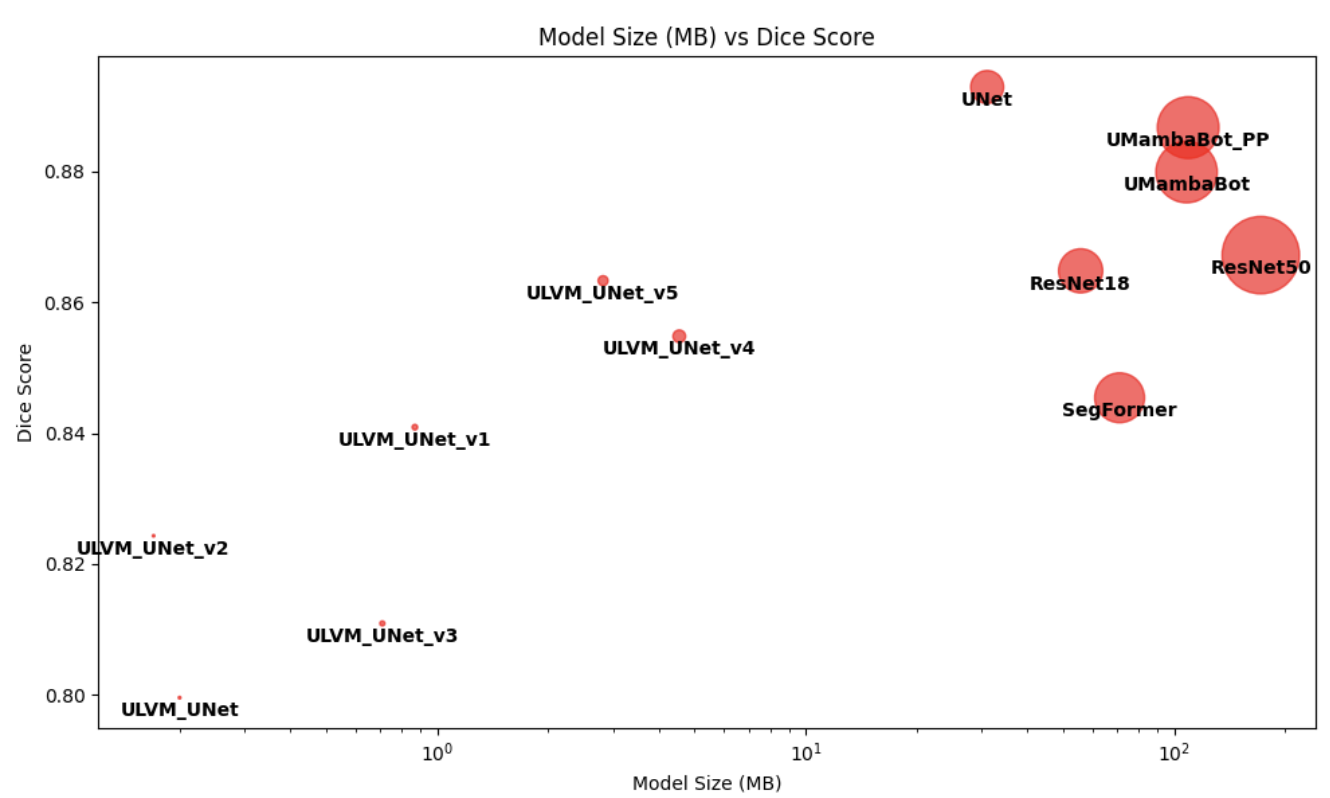
\includegraphics[width=\columnwidth]{imgs/balls.png}
    \caption{A scatter plot of Dice Score vs model size in MegaBytes. The points are scaled to help represent size.}
    \label{fig:balls}
\end{figure}
\begin{figure}[!t]
    \centering
    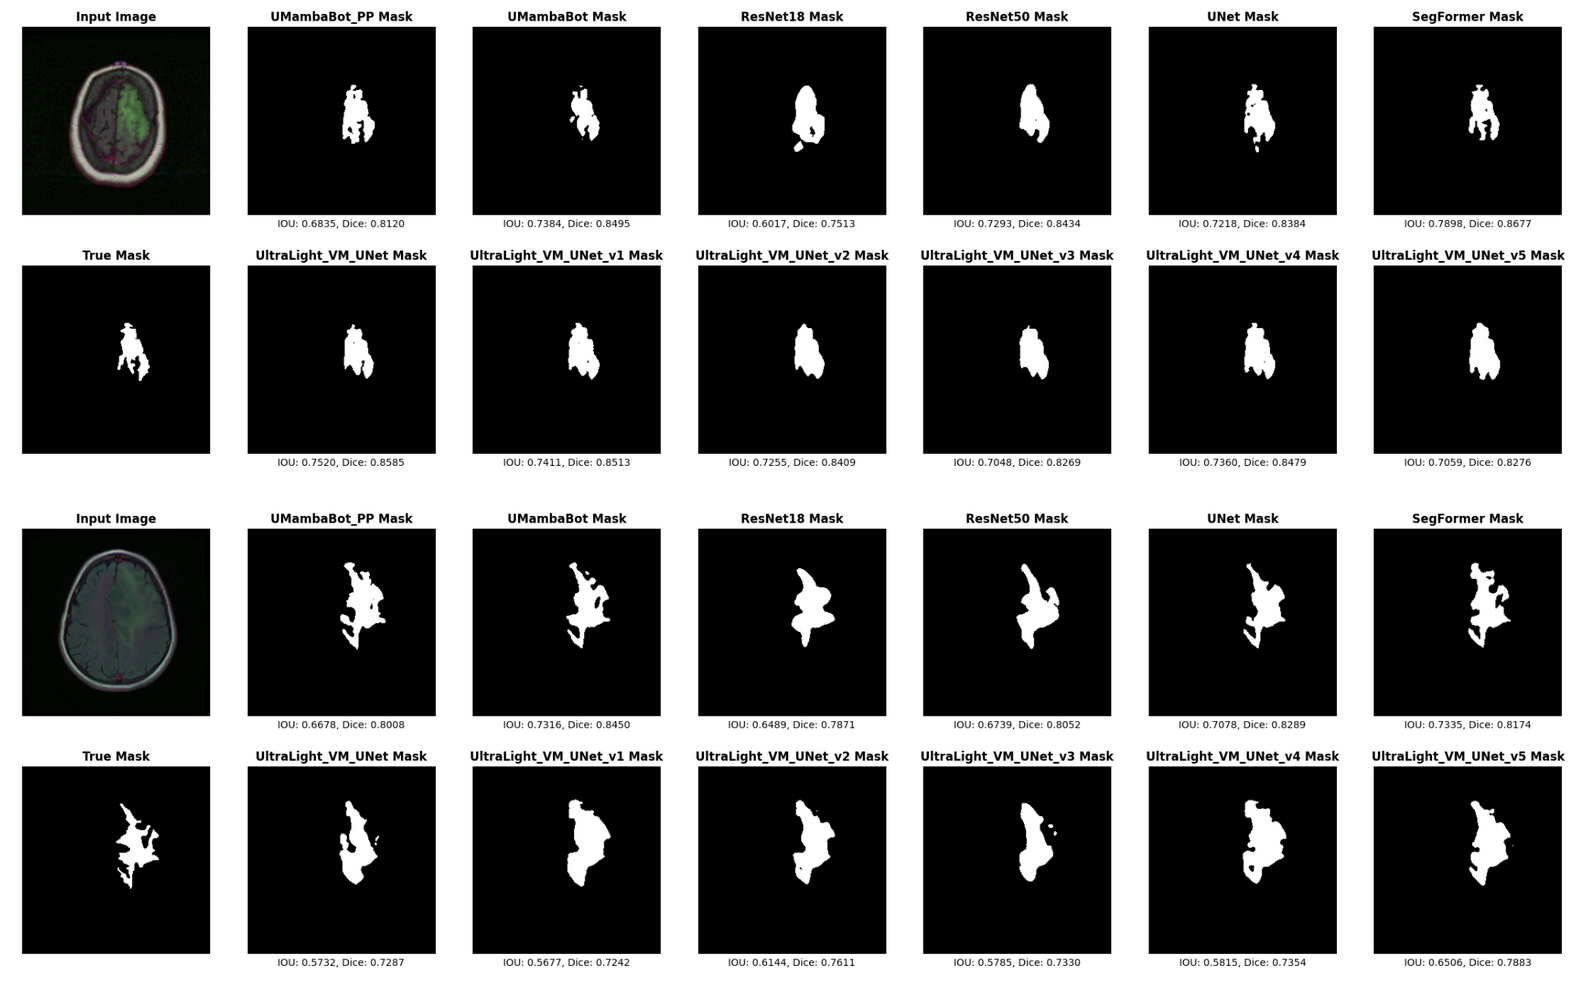
\includegraphics[width=\columnwidth]{imgs/masks.png}
    \caption{Example segmentations.}
    \label{fig:segs}
\end{figure}

\section{Conclusion}

In this work, we explored the application of Structured State Space Sequence Models (SSMs), particularly the Mamba architecture, for tumor segmentation from brain MRI scans. The Mamba architecture leverages selective state spaces, enabling efficient and effective segmentation while maintaining linear scalability.

Our experiments and comparisons with state-of-the-art (SOTA) models demonstrate the potential of the Mamba-based approach in both model size and segmentation accuracy. The smallest model, ULVM\_Net\_v2, achieved a compelling dice score of 0.8243 with only 0.042M parameters, outperforming the larger ResNet50 model (42.9M params) with a dice score of 0.8672.

While the traditional U-Net model achieved the highest dice score of 0.8929, our PP-UMamba model closely followed with a dice score of 0.8867. Notably, our Mamba-based UMambaBot\_PP and UMambaBot models outperformed the Segformer transformer model, indicating the potential of Mamba-based approaches to surpass transformer-based models for this task.

We were able to make the ultra-light model smaller and more accurate on our task, further proving the potential of Mamba-based systems that prioritize compactness and efficiency. The selective state spaces and parallel processing strategies employed in our models enabled us to strike a balance between model size and segmentation accuracy.

Overall, this work contributes to the exploration of Structured State Space Sequence Models for medical image segmentation tasks. The Mamba architecture's ability to capture long-range dependencies while maintaining linear scalability positions it as a promising alternative to traditional convolutional and transformer-based approaches, especially in resource-constrained environments.

Future work could involve further refinements and optimizations of the Mamba-based models, as well as their application to other medical imaging modalities and segmentation tasks. Additionally, investigating the interpretability and robustness of these models could provide valuable insights for their deployment in real-world clinical settings.

\begin{thebibliography}{00}
\bibitem{ronneberger2015unet} O. Ronneberger, P. Fischer, and T. Brox, "U-Net: Convolutional Networks for Biomedical Image Segmentation," arXiv:1505.04597 [cs.CV], 2015.

\bibitem{vaswani2023attention} A. Vaswani et al., "Attention Is All You Need," arXiv:1706.03762 [cs.CL], 2023.

\bibitem{gu2022efficiently} A. Gu, K. Goel, and C. Ré, "Efficiently Modeling Long Sequences with Structured State Spaces," arXiv:2111.00396 [cs.LG], 2022.

\bibitem{gu2023mamba} A. Gu and T. Dao, "Mamba: Linear-Time Sequence Modeling with Selective State Spaces," arXiv:2312.00752 [cs.LG], 2023.

\bibitem{bakas2019identifying} S. Bakas et al., "Identifying the Best Machine Learning Algorithms for Brain Tumor Segmentation, Progression Assessment, and Overall Survival Prediction in the BRATS Challenge," arXiv:1811.02629 [cs.CV], 2019.

\bibitem{U-Mamba} J. Ma, F. Li, and B. Wang, "U-Mamba: Enhancing Long-range Dependency for Biomedical Image Segmentation," arXiv:2401.04722 [cs.CV], 2024.

\bibitem{rombach2021highresolution} R. Rombach, A. Blattmann, D. Lorenz, P. Esser, and B. Ommer, "High-Resolution Image Synthesis with Latent Diffusion Models," arXiv:2112.10752 [cs.CV], 2021.

\bibitem{DBLP:journals/corr/abs-2006-11239} J. Ho, A. Jain, and P. Abbeel, "Denoising Diffusion Probabilistic Models," CoRR, vol. abs/2006.11239, 2020. [Online]. Available: https://arxiv.org/abs/2006.11239

\bibitem{DBLP:journals/corr/HeZRS15} K. He, X. Zhang, S. Ren, and J. Sun, "Deep Residual Learning for Image Recognition," CoRR, vol. abs/1512.03385, 2015. [Online]. Available: http://arxiv.org/abs/1512.03385

\bibitem{zhang2022segvit} B. Zhang et al., "SegViT: Semantic Segmentation with Plain Vision Transformers," arXiv:2210.05844 [cs.CV], 2022.

\bibitem{dosovitskiy2021image} A. Dosovitskiy et al., "An Image is Worth 16x16 Words: Transformers for Image Recognition at Scale," arXiv:2010.11929 [cs.CV], 2021.
\bibitem{ultralightvmunet} R. Wu, Y. Liu, P. Liang, and Q. Chang, “UltraLight VM-UNet: Parallel Vision Mamba Significantly Reduces Parameters for Skin Lesion Segmentation.” Accessed: Apr. 20, 2024. [Online]. Available: https://arxiv.org/pdf/2403.20035.pdf
\bibitem{zhao2017pyramid}
H. Zhao, J. Shi, X. Qi, X. Wang and J. Jia, "Pyramid Scene Parsing Network," 2017 IEEE Conference on Computer Vision and Pattern Recognition (CVPR), 2017, pp. 6230-6239, doi: 10.1109/CVPR.2017.660.
\bibitem{dataset} “Brain MRI segmentation,” www.kaggle.com. https://www.kaggle.com/datasets/mateuszbuda/lgg-mri-segmentation
\end{thebibliography}
\end{document}
